\documentclass[10pt]{article}

\input{../preambule}
\input{../styles}
\input{../bas_de_page_quatrieme} 

%%%%%%%%%%%   Marges de pages  %%%%%%%%%%%%%%%% 
 \usepackage{geometry}
 \geometry{top=2cm, bottom=0cm, left=2cm , right=2cm}
%%%%%%%%%%%%%%%%%%%%%%%%%%%%%%%%%%%%%%%%%%%%%%%
\usepackage{eurosym}
%%%%%%%%%%%%%%%  Indentation  %%%%%%%%%%%%%%%%%%
\parindent=0pt
%%%%%%%%%%%%%%%%%%%%%%%%%%%%%%%%%%%%%%%%%%%%%%%%
\usepackage{eurosym}

\begin{document}

%%%%%%%%%%%%%%%%%%%%%%%%%%%%%%%%%%%%%%%%%%%%%%%
%%%%		 Titre encadré
%%%%%%%%%%%%%%%%%%%%%%%%%%%%%%%%%%%%%%%%%%%%%%%
\begin{encadrementombre}{Thème 5: Proportionnalité}
{\LARGE Proportionnalité }\\

%% Laisse la ligne vide ci-dessus
{\Large Gestion de données}
\end{encadrementombre}


%%%%%%%%%%%%%%%%%%%%%%%%%%%%%%%%%%%%%%%%%%%%%%%
%%%%		 Corps du document
%%%%%%%%%%%%%%%%%%%%%%%%%%%%%%%%%%%%%%%%%%%%%%%

%%%%%%%%%%%%%%%%%%%%%%%%%%%%%%%%%%%%%%%%%%%%%%%
%%%% \renewcommand{\arraystretch}{1.8}
\definecolor{shadecolor}{gray}{0.9}
%%%%%%%%%%%%%%%%%%%%%%%%%%%%%%%%%%%%%%%%%%%%%%%
%%%%%%%%%%%   Hauteur de ligne  %%%%%%%%%%%%%%%%
{\setlength{\baselineskip}{1.5\baselineskip}
%%%%%%%%%%%%%%%%%%%%%%%%%%%%%%%%%%%%%%%%%%%%%%%%

\section{Pour démarrer le thème: Quelques rappels (voir Sesamath)}
 
\begin{enumerate}
\item On sait que $6 kg$ de pommes coûte $9,60$ \euro{}. Combien coûte $7kg$ de pommes?
\begin{enumerate}	
	\item On ne peut pas savoir
	\item $\frac{9,60 \times 7}{6}$ \euro{}
	\item $7 \times 1,60$\euro{}
	\item $9,60 \times \frac{7}{6}$
\end{enumerate}
\item Six cédéroms coûtent $102$ \euro{}. Combien coûtent $15$ cédéroms?
\begin{enumerate}	
	\item $102 \times 2 +102 \div 2$
	\item $102 \times \frac{15}{6}$
	\item $\frac{102}{6} \times 15$
	\item $260$
\end{enumerate}  
\item Les tableaux suivants sont-ils des tableaux de proportionnalité?
\begin{enumerate}	
	\item 
	\newcolumntype{R}[1]{>{\raggedleft\arraybackslash}b{#1}}
	\newcolumntype{L}[1]{>{\raggedright\arraybackslash}b{#1}}
	\newcolumntype{C}[1]{>{\centering\arraybackslash}b{#1}}
	
	\begin{tabular}{|L{2cm}||C{1cm}|C{1cm}|C{1cm}|}
	\hline Masse en $kg$&$15$&$33,75$\\
	\hline Prix en \euro{}&$4$&$9$\\
	\hline
	\end{tabular}	
	\item 
	\newcolumntype{R}[1]{>{\raggedleft\arraybackslash}b{#1}}
	\newcolumntype{L}[1]{>{\raggedright\arraybackslash}b{#1}}
	\newcolumntype{C}[1]{>{\centering\arraybackslash}b{#1}}
	
	\begin{tabular}{|L{3cm}||C{1cm}|C{1cm}|C{1cm}|}
	\hline Distance en $m$&$3$&$4,5$\\
	\hline Durée en $mn$&$12,2$&$18,4$\\
	\hline
	\end{tabular}
	\item 
	\newcolumntype{R}[1]{>{\raggedleft\arraybackslash}b{#1}}
	\newcolumntype{L}[1]{>{\raggedright\arraybackslash}b{#1}}
	\newcolumntype{C}[1]{>{\centering\arraybackslash}b{#1}}
	
	\begin{tabular}{|L{2cm}||C{1cm}|C{1cm}|C{1cm}|}
	\hline Volume en $L$&$4$&$5,2$\\
	\hline Prix en \euro{}&$5,5$&$7,15$\\
	\hline
	\end{tabular}
\end{enumerate}

\item Complète les tableaux suivants en sachant qu'ils sont des tableaux de proportionnalité:
\begin{enumerate}	
	\item 
	\newcolumntype{R}[1]{>{\raggedleft\arraybackslash}b{#1}}
	\newcolumntype{L}[1]{>{\raggedright\arraybackslash}b{#1}}
	\newcolumntype{C}[1]{>{\centering\arraybackslash}b{#1}}
	
	\begin{tabular}{|L{2cm}||C{1cm}|C{1cm}|C{1cm}|}
	\hline Masse en $kg$&$11$&$...$\\
	\hline Prix en \euro{}&$4$&$15,2$\\
	\hline
	\end{tabular}
	
	\item 
	\newcolumntype{R}[1]{>{\raggedleft\arraybackslash}b{#1}}
	\newcolumntype{L}[1]{>{\raggedright\arraybackslash}b{#1}}
	\newcolumntype{C}[1]{>{\centering\arraybackslash}b{#1}}
	
	\begin{tabular}{|L{3cm}||C{1cm}|C{1cm}|C{1cm}|}
	\hline Distance en $m$&$3$&$4,5$\\
	\hline Durée en $mn$&$12,87$&$...$\\
	\hline
	\end{tabular}
	
	\item 
	\newcolumntype{R}[1]{>{\raggedleft\arraybackslash}b{#1}}
	\newcolumntype{L}[1]{>{\raggedright\arraybackslash}b{#1}}
	\newcolumntype{C}[1]{>{\centering\arraybackslash}b{#1}}
	
	\begin{tabular}{|L{2cm}||C{1cm}|C{1cm}|C{1cm}|}
	\hline Volume en $L$&$...$&$5,4$\\
	\hline Prix en \euro{}&$23,4$&$17,55$\\
	\hline
	\end{tabular}
\end{enumerate}
\item Complète les tableaux de proportionnalité suivants:
	\begin{enumerate}	
	\item 
	\newcolumntype{R}[1]{>{\raggedleft\arraybackslash}b{#1}}
	\newcolumntype{L}[1]{>{\raggedright\arraybackslash}b{#1}}
	\newcolumntype{C}[1]{>{\centering\arraybackslash}b{#1}}
	
	\begin{tabular}{|L{2cm}||C{1cm}|C{1cm}|C{1cm}|}
	\hline Masse en $kg$&$11$&$...$\\
	\hline Prix en \euro{}&$4$&$12$\\
	\hline
	\end{tabular}
	
	\item 
	\newcolumntype{R}[1]{>{\raggedleft\arraybackslash}b{#1}}
	\newcolumntype{L}[1]{>{\raggedright\arraybackslash}b{#1}}
	\newcolumntype{C}[1]{>{\centering\arraybackslash}b{#1}}
	
	\begin{tabular}{|L{3cm}||C{1cm}|C{1cm}|C{1cm}|}
	\hline Distance en $m$&$3,9$&$4,5$\\
	\hline Durée en $mn$&$23,01$&$...$\\
	\hline
	\end{tabular}
	
	\item 
	\newcolumntype{R}[1]{>{\raggedleft\arraybackslash}b{#1}}
	\newcolumntype{L}[1]{>{\raggedright\arraybackslash}b{#1}}
	\newcolumntype{C}[1]{>{\centering\arraybackslash}b{#1}}
	
	\begin{tabular}{|L{2cm}||C{1cm}|C{1cm}|C{1cm}|}
	\hline Volume en $L$&$...$&$6$\\
	\hline Prix en \euro{}&$21$&$18$\\
	\hline
	\end{tabular}	
\end{enumerate} 
\item Quels sont les graphiques qui illustrent une situation de proportionnalité?
	\begin{enumerate}	
	\item 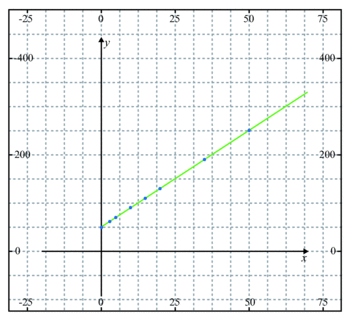
\includegraphics[scale=0.3]{question6_a.eps} \textbf{(b)} 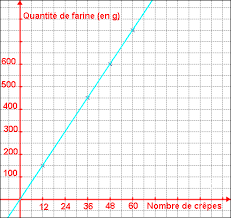
\includegraphics[scale=0.43]{question6_c.eps}  		\textbf{(c)} 
	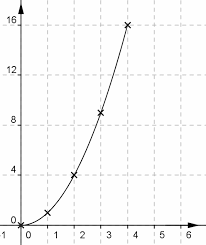
\includegraphics[scale=0.4]{question6_b.eps} 
	\end{enumerate}
\end{enumerate}

\newpage


%%%%%%%%%%%%%%%%%%%%%%%%%%%%%%%%%%%%%%%%%%%%%%%%%%%%%%%
%     Notions
%%%%%%%%%%%%%%%%%%%%%%%%%%%%%%%%%%%%%%%%%%%%%%%%%%%%%%%

\section{Cours}
\subsection{Généralités et rappels}
\begin{shaded}
\begin{Pp}
Dans une situation de proportionnalité, la \textbf{\og quatrième proportionnelle \fg{}} est le quatrième nombre, noté $x$, que l'on peut calculer à partir des trois autres $a$, $b$ et $c$ connus. Ainsi, si le tableau suivant est un tableau de proportionnalité 
\newcolumntype{R}[1]{>{\raggedleft\arraybackslash}b{#1}}
	\newcolumntype{L}[1]{>{\raggedright\arraybackslash}b{#1}}
	\newcolumntype{C}[1]{>{\centering\arraybackslash}b{#1}}
	
	\begin{tabular}{|L{2cm}||C{1cm}|C{1cm}|C{1cm}|}
	\hline quantité A&$a$&$x$\\
	\hline quantité B&$b$&$c$\\
	\hline
	\end{tabular}
, alors: $\frac{c}{x}=\frac{b}{a}$ ou encore $a \times c = b \times x$ (\textbf{égalité des produits en croix}) et donc $x= \frac{ac}{b}$
\end{Pp}
\end{shaded}
   
\begin{Ex}   
Calculer le prix $x$ en \euro{} d'un écran de $1 300 000$ COP sachant que $300$ \euro{} correspond à $967200$ COP.
\\ On  utilise l'égalité  $\frac{1300000}{x}=\frac{967200}{300}$ soit $1300000 \times 300 = 967200 \times x$ et donc $x= \frac{1300000\times 300}{967200}$. On obtient environ $403$ \euro{}.  
\end{Ex}

\begin{shaded}
\begin{Pp}
\begin{enumerate}
\item Une situation de proportionnalité est représentée graphiquement par des points qui sont alignés sur une droite qui passe par l'origine du repère.
\item Réciproquement, si deux grandeurs sont représentée graphiquement par une droite qui passe par l'origine du repère, alors ces deux grandeurs sont proportionnelles.
\end{enumerate}
\end{Pp}
\end{shaded}

\begin{Pv}
	-A faire en classe-
\end{Pv}   

\begin{Ex} 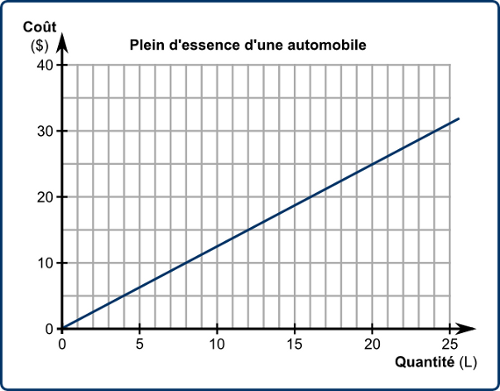
\includegraphics[scale=0.6]{SituationProportionnelleGraphique.eps} 
 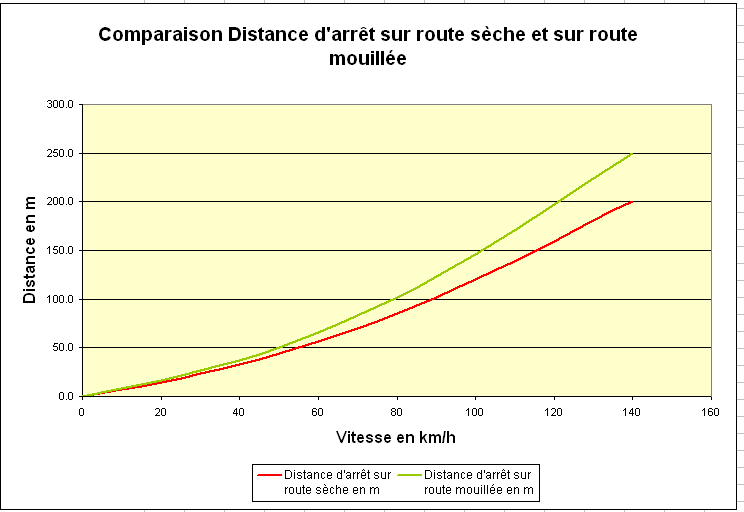
\includegraphics[scale=0.29]{graphique_nonproportionnalite.eps}
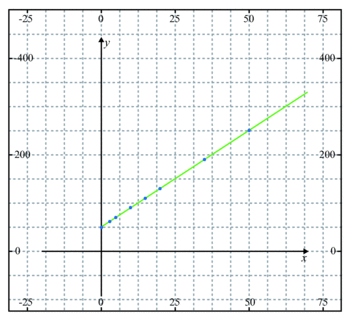
\includegraphics[scale=0.36]{question6_a.eps} 
 \end{Ex}

\subsection{Pourcentage}

\begin{Df}
Un \textbf{pourcentage} est une écriture fractionnaire dont le dénominateur est égal à $100$. On utilise la notation $x \%$ qui signifie $\frac{x}{100}$
\end{Df}

\begin{Ex}   
\begin{itemize}
\item Dans une classe de $27$ élèves, il y a $19$ filles. Quel pourcentage de la classe représente les filles dans cette classe?
\\La proportion de filles dans cette classe est $\frac{19}{27}$, soit environ $0,7037$ soit $70,37 \%$
\item En France, environ $10,3 \%$ de la population active est au chômage.
sachant que la population active est de $28,6$ millions, calculer le nombre de chômeurs arrondi au millier.
\end{itemize}
\end{Ex}

\begin{Rq}
En économie,une augmentation de \og 7 points \fg{} signifie une augmentation de $7 \%$ 
\end{Rq}

\subsection{Vitesse moyenne}

\begin{Df} 
Si $t$ est le temps écoulé pour parcourir la distance $d$, alors la \textbf{vitesse moyenne} sur ce trajet est $v=\frac{d}{t}$
\end{Df}

\begin{Rq}   
\begin{itemize}
\item On a aussi les relations $d=v \times t$ et $t=\frac{d}{v}$
\item Les vitesses sont souvent exprimées en $m.s^{-1}$ ou en $km.h^{-1}$ mais il existe d'autre unité de vitesse comme les tour.min$^{-1}$, \ldots{}
\item Pour convertir les unités, on rappelle que $1h=60$min$=3600s$ et que $1$km$=1000$m$=1000000$mm
\end{itemize}
\end{Rq}

\begin{Ex}
\begin{enumerate}
\item Calculer la vitesse moyenne de U.Bolt lors de son record du $100 m$ en $9'58''$
\item Sachant qu'un avion vole à une vitesse moyenne de $900 km.s^{-1}$, quel distance parcours un avion en $1 mn$?
\item Sachant que Gabin cours à une vitesse de pointe de $20 km.h^{-1}$, et qu'il part ce matin en retard de chez lui à $8h17min$, arrivera-t-il à l'heure à l'école qui se trouve à $4,5 km$ et qui commence à $8h30$min?
\end{enumerate}
\end{Ex}



\newpage



\section{Quelques exercices}
\begin{Exo}
Sur la route, lorsqu'un évènement imprévu survient, le conducteur
réagit avec un temps de retard d'environ 1 seconde et la voiture
parcourt encore une certaine distance qui dépend de la vitesse à
laquelle roule le véhicule.\\Le tableau ci-dessous indique différents
résultats de relevés effectués par La Gendarmerie Nationale.
\begin{center}
\begin{tabularx}{8cm}{|X|c|c|c|}
\hline
Vitesse en km/h&50&70&100\\
\hline
Distance parcourue pendant le temps de réaction&14&19,6&28\\
\hline
\end{tabularx}
\end{center}
\begin{enumerate}
\item Ce tableau correspond-il à une situation de proportionnalité ?
\item Quelle est la distance parcourue pendant le temps de réaction si
l'on roule à 90~km/h ? Et à 130~km/h ?\par{\em On
  poursuivra le tableau de la question précédente pour y indiquer ces vitesses.}
\item \`A quelle vitesse roule-t-on si la distance de réaction est
  30,8~m ?\par{\em On poursuivra le tableau de la question précédente
    pour y indiquer cette distance.}
\end{enumerate}
\end{Exo}

\begin{Exo}
\begin{center}
\begin{tabularx}{0.75\linewidth}{|c|X|X|X|X|}
\hline
Article&Prix avant soldes (en \euro{})&
Remise en \%&Remise en \euro{}&Nouveau prix (en \euro{})\\
\hline
Pantalon&\multicolumn{1}{c|}{29}&\multicolumn{1}{c|}{15}&&\\
\hline
Chemise&\multicolumn{1}{c|}{22}&&\multicolumn{1}{c|}{4,4}&\\
\hline
Veste&&\multicolumn{1}{c|}{20}&&\multicolumn{1}{c|}{55,2}\\
\hline
\end{tabularx}
\end{center}
 On a relevé, dans le tableau ci-dessus, les différents prix
 d'articles en soldes.\\Recopie et complète le tableau (tous les
 calculs nécessaires doivent apparaître sur la copie).
\end{Exo}

\begin{Exo}
Il a été demandé aux familles de deux villages voisins $S$ et $T$ de
répondre à la question suivante :\og \^Etes-vous favorable à
l'aménagement d'une piste cyclable entre les deux villages ?\fg
\begin{enumerate}
\item
\begin{enumerate}
\item Dans le village $S$, 60\% des 135 familles consultées ont
répondu \og oui\fg.\par Combien de familles, dans ce village, sont
favorables à ce projet ?
\item Dans le village $T$, il y a 182 réponses favorables sur les
$416$ familles consultées.\par Quel est le pourcentage de \og oui\fg\
pour le village $T$ ?
\end{enumerate}
\item La décision d'aménager la piste cyclable ne peut être prise
qu'avec l'accord de la majorité des familles de l'ensemble des deux
villages. La piste cyclable sera-t-elle réalisée ?
\end{enumerate}
\end{Exo}

\begin{Exo}
On sait que la superficie du globe est de 510 millions de km$^2$.
\begin{enumerate}
\item Recopie et complète le tableau suivant :
\\\begin{tabular}[c]{|c|c|c|}
 \hline Océan & superficie (en millions de km$^2$) & \% de la 
 superficie totale de la terre \\  
 \hline Pacifique & 180 &  \\  
 \hline Atlantique & 106 & \\
 \hline Indien & 75 &  \\
 \hline Total & & \\
 \hline 
\end{tabular}
 \item Le nom de la planète bleue pour la terre est-il justifié ?
 \item La mer méditerranée a une superficie de 2,5 millions de km$^2$.
   \begin{enumerate}
      \item Exprime en pourcentage sa superficie par rapport à celle 
      de l'océan atlantique.
      \item Calcule le pourcentage de la superficie du globe par rapport 
      à celle du globe.    
    \end{enumerate}  
\end{enumerate}
\end{Exo}

\begin{Exo}
Dans une classe de 22 élèves, il y a 12 filles et 10 garçons.
50\% des filles et 70\% des garçons mangent à la cantine.
\begin{enumerate}
\item Combien de filles mangent à la cantine ?
%\correction{${50\over100}\times12=6$}
\item Combien de garçons mangent à la cantine ?
%\correction{${70\over100}\times10=7$}
\item Combien d'élèves mangent à la cantine dans cette classe ?
%\correction{$6+7=13$}
\item Quel pourcentage cela représente-t-il ?
%\correction{${13\over22}\times100\approx59$.\\
%$59\%$ des élèves environ mangent à la cantine.}
\end{enumerate}
\end{Exo}

\begin{Exo}
Une voiture doit effectuer un trajet de 100 km.\\
Pendant les 50 premiers kilomètres, il roule à la vitesse de 80 km/h.\\
Pendant les 50 derniers kilomètres, il roule à la vitesse de 100 km/h.
\begin{enumerate}
\item Combien de temps a-t-il mis pour effectuer les 50 premiers kilomètres ?
%\correction{$50\div80=0,625$ heures, soit $0,625\times60=37,5$ minutes.}
\item Combien de temps a-t-il mis pour effectuer les 50 derniers kilomètres ?
%\correction{$50\div100=0,5$ heures, soit $0,5\times60=30$ minutes.}
\item Combien de temps a-t-il mis en tout ?
%\correction{$0,625+0,5=1,125$ heures.}
\item Quelle a été sa vitesse moyenne sur le trajet ?
%\correction{$100\div1,125\approx88,9$ km/h.}
\end{enumerate}
\end{Exo}


\begin{Exo}
\begin{enumerate}
\item Si on augmente le prix d'un article de $20\%$ et qu'un mois plus tard effectue une baisse de $20\%$, le prix de cet article va-t-il revenir à son prix initial? Expliquer
\item De combien doit-on baisser pour compenser une hausse de $20\%$?
\end{enumerate}
\end{Exo}
  
\begin{Exo}
\begin{enumerate}
\item En 1971, à la course automobile des 24 heures du Mans, une
  Porsche a parcouru 5\,335,313~km. Calcule sa vitesse moyenne en
  km/h.
\item En 1990, le tracé de la piste est changé et en 1993, une Peugeot
  905 a battu le record de la distance sur ce nouveau parcours à une
  vitesse moyenne de 213,58~km/h.\\Quelle distance a parcourue cette
  voiture ?
\item En 1997, le tracé ayant été encore modifié pour raisons de
  sécurité, il aurait fallu 26~h~7~min~47~s à la Porsche
  victorieuse pour parcourir la même distance que la voiture
  gagnante de 1971. \`A quelle vitesse moyenne a roulé le vainqueur en
  1997 ? Quelle distance a-t-il parcourue en 24~h ?
\end{enumerate} 
%@Commentaire: Utilisation de la formule de calcul de vitesse avec les trois possibilités. Attention aux conversions d'unités de temps.
\end{Exo}

\begin{Exo}
\par {\em Champion de France Amateurs -- Cyclisme : Pauriol - Les 164,4~km en 4~h~7~min~20~s (39,881~km/h).}
\par
Justifie par un calcul la vitesse moyenne donnée.
\end{Exo}

\begin{exo}\textbf{(Problème de train)}
\\Le TGV \og Nord \fg{} part de Lille à $10h20$ vers Paris à la vitesse de $227$km.h$^{-1}$ et le TGV \og Sud \fg{} part de Paris à $10h30$ vers Lille à la vitesse de $239$km.h$^{-1}$. La distance Lille-Paris est environ $220$ km par le train. Ces deux trains vont-ils se croiser avant $10h53$?
\end{exo}


\begin{exo}\textbf{Problème de train (bis)}
\\Le train A roule à la vitesse moyenne de $100$ km.h$^{-1}$ et le train B roule à la vitesse moyenne de $120$ km.h$^{-1}$. A $9$h, le train A part de Lille pour Lyon et le train B part de Lyon pour Lille. La distance Lille-Lyon est $660$ km.
\begin{enumerate}
\item A quelle distance de Lille se trouveront ces trains à $11$h? A $11$h$30$?
\item A quelle heure les trains A et B vont-ils se croiser?
\end{enumerate}
\end{exo}
   




      
\newpage



\end{document}